\chapter{Analysis}
This chapter focuses mainly on the analysis of the empirical data from an academic perspective, to make fact based conclusions. The section begins with the Interview insights, where based on the interview transcripts the KPIs are analysed. In the next section, the inferences from the survey are drawn and discussed. Later, the answer to all the three research questions have been analysed and presented.
 
\section{ Interview insights }
The interviews with the KPI owners and the directors gave insights on the present condition of the KPIs such as how they were framed, how they were measured and their characteristics. Based on the literature study conducted, various ideal characteristics of the KPIs have been gathered. The interview conclusions are compared with the academic perspectives of the KPIs to understand if the present KPIs satisfy all the characteristics or if they need any improvement. 
This analysis is done in two phases,\\ 
\begin{itemize}
    \item Initially, each KPI is analyzed using AHP(Analytical Hierarchical Process) and SMART framework to understand the order or rank in which those KPIs satisfy a particular characteristic.\\  
    \item In the second phase the KPIs are classified as leading or lagging.\\   
\end{itemize}
 The phases are explained below:

\subsection{KPI Characteristics analysis by SMART and AHP}
Based on the article by Shahin(2007), a combination of SMART and AHP was used to analyze the KPIs to understand if they meet the SMART criteria. The AHP was conducted using the interview data and observations. \\
The following KPIs were chosen to perform the AHP, as understood from the empirical data these were given more importance. The list of chosen KPIs are : \\

\begin{itemize}
    \item QJ lead time
    \item PROTUS
    \item DCN Release
    \item Project Deliveries
    \item Test cell delivery precision
    \item Financial KPI´s
    \item Net operational expenses \% of latest decided budget CAP

\end{itemize}
AHP for each of the criteria of SMART was conducted and the rating/ ranks of the KPIs were obtained as follows: 
\subsubsection{Specific}
As mentioned in the theory, this criteria meant the KPI needed to be precise and clear. Detailed study on objective behind these KPIs, the way they are measured etc were used to conduct the AHP, and the Ranks of the KPIs were derived as shown in figure \ref{fig:6.1}.\\

\begin{figure}[H]
    \centering
    \captionsetup{justification=centering, margin=2cm}
    \vspace{1cm}
    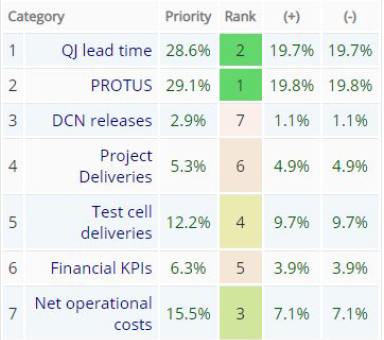
\includegraphics[width=10cm, height=7cm]{figure/auxiliary/fig61.PNG}
    \caption{KPI Ranking based on Specific character}
    \label{fig:6.1}
\end{figure}
%put fig 6.1


This analysis aimed at verifying which KPI was most specific and rank them accordingly. From the interviews and this analysis we see that PROTUS and QJ lead time were the most precise and specific KPI with 29.1\% & 28.5\% priority respectively. It was also being followed regularly by all the employees. They have 2 different measures under them, though one of them needed revision according to the interviewees, it was still very specific and related to the work. 
The least specific, as seen in the Fig. was DCN Releases with a priority rating of 2.9\%. From the interviews it could be recollected that this KPI needed clearer definitions like agreed completed date and had to be more specific in its definitions and targets.Project deliveries was the second least with 5.3\% priority, as understood from the interviews the KPIs under this were vague, abstract and complicated. \\
Hence, the data from the interviews and the definitions of the KPIs contributed to classify how specific the KPIs are.\\

\subsubsection{Measurable}
Using the description as mentioned in theory the importance ratings were given to each KPI, and the following result was obtained as shown in figure \ref{fig:6.2}:\\

%put fig 6.2
\begin{figure}[H]
    \centering
    \captionsetup{justification=centering, margin=2cm}
    \vspace{1cm}
    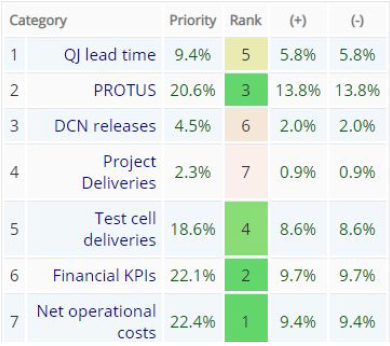
\includegraphics[width=10cm, height=7cm]{figure/auxiliary/fig62.PNG}
    \caption{KPI Ranking based on Measurable character}
    \label{fig:6.2}
\end{figure}

The “Net operational costs” and “Financial KPIs” were relatively more measurable with a priority rating of approximately 22\%. They had a clear definition for calculations and smoother ways to collect data. \\
The least ranked was again the Project deliveries with 2.3\% priority rating. The measures were vague and complicated to make conclusions as mentioned in the interviews, hence it has the lowest rank. Similar issue was faced with measuring Engineering direct runners under DCN releases as measures were easy to manipulate and the employees thought the measures were unreliable. \\

\subsubsection{Attainable and Realistic}
These criteria had a similar meaning as defined in the theory, hence the AHP was conducted by keeping both attainability and realistic nature in mind. The data from 2018 KPIs were used with more focus, to input the ratings. The ranks were obtained from this analysis as depicted in figure \ref{fig:6.3}:\\
\begin{figure}[H]
    \centering
    \captionsetup{justification=centering, margin=2cm}
    \vspace{1cm}
    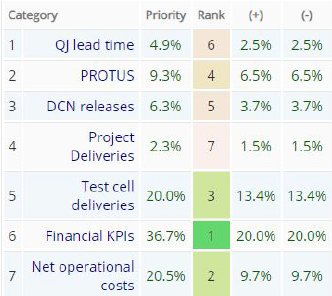
\includegraphics[width=10cm, height=7cm]{figure/auxiliary/fig63.PNG}
    \caption{KPI Ranking based on Attainable and Realistic character}
    \label{fig:6.3}
\end{figure}
%put fig 6.3
The financial KPIs and net operational cost were the first two with 36.7\% and 20.5\% priority. They had achievable targets, though there were out of target value in few months they did not seem unrealistic. But Project deliveries had the least rank. The targets were not realistic. Depending on the projects it was difficult to compare them or set the same target. The real quality of the project was not being measured, and just having the current KPIs was not a good goal. The second least rated was QJ Lead time, though this KPI had the right objective and measures, the targets set were not attainable. Throughout the year this KPI was marked red, there was no analysis done to set attainable targets, thus making it the second least attainable KPI.\\

\subsubsection{Time Sensitive}
Keeping the definition mentioned in theory the ranks were obtained for each KPI as depicted in figure \ref{fig:6.4}\\


Most of the KPIs were time sensitive, but the highlight was the KPI with least rank i.e Project deliveries. As per the interviews, though the KPI was supposed to be measured and analyzed monthly, the data was updated rarely. One of the KPIs under project deliveries was measured only once in the year 2018. Hence this KPI received the least priority rating of 5.9\%
Engineering direct runners under DCN releases on the other hand got the second least rating as the release time changed and hence does not provide complete reliability in time factor. \\
\begin{figure}[H]
    \centering
    \captionsetup{justification=centering, margin=2cm}
    \vspace{1cm}
    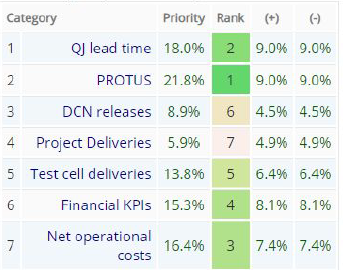
\includegraphics[width=10cm, height=7cm]{figure/auxiliary/fig64.PNG}
    \caption{ KPI Ranking based on Time Sensitivity}
    \label{fig:6.4}
\end{figure}
%put fig 6.4


\subsection{Leading and Lagging categorization}
Apart from the analysis of SMART, it is also necessary to know if the KPIs were leading or Lagging. Based on the definition of leading and lagging KPIs given by Manuele(2009), PE sweden  KPIs were divided into both categories. \% of gross expenses is categorized as leading, since the budget for the year is known and tracking monthly expenses would help predict budget overrun in future, hence making it a leading KPI in this case. Whereas, GPOT is categorized as a lagging KPI, since the value is got only after a gate is passed and if it is not passed it cannot be fixed for that month or period of time. Thus, with similar understanding all the twenty three KPIs are categorized as represented in Table 6.1 :
\begin{table}[h]
    \centering
    \captionsetup{justification=centering, margin=2cm}
    \scalebox{0.9}{%
    \begin{tabular}{|c|c|c|c|c|c|c|}
    \hline
  % \begin{align}
    \textbf{Leading Indicators} & \textbf{Lagging indicators} \\
    \hline
    \% of gross expenses & NEW to Market ready\\\hline
     NEW to Containment action & Inflow vs. solved (status 10 / status 8), 3m rolling\\\hline
     POTUS age in status 10 - 3 [days] & Trust and Passion KPIs\\\hline
     Projects with fulfilled need maturity & Patents: No. of ideas \\\hline
     QDCCF fulfilment & No. of closed Kanban initiatives (incl VGAS actions)\\\hline
     DVG Certified Knowledge & Engineering Direct Runners\\\hline
     Chargeability & DCN released on time\\\hline
     \% of gross expenses & GPOT - Gates Passed On Time \\\hline
     \% of latest decided budget CAP & Test Cell Delivery Precision\\\hline
     - & Total time reported in SCORE\\\hline
     - & Hourly rate [SEK]\\\hline
   %  \end{align}
    \end{tabular}}
    \caption{ Categorization of KPIs into Leading and Lagging }
   \label{tab:lead_Lag}
\end{table}

%https://docs.google.com/document/d/13o1zj7z6Jqv_lOrmzcdZb1IeIuYddI_a0uvVVYpKcR8/edit
From the table \ref{tab:lead_Lag} above, it is seen that most of the KPIs were lagging indicators, which means the results were analyzed only after the damage was done. Peterson(2014) mentions that “KPIs are meant to provide a compliment of leading and lagging indicators that effectively communicate the day to day operations of the business.”, hence there needs to be a right balance of both leading and lagging KPIs to drive the business.

\section{ Survey insights }
In this section ,the inferences from the survey is drawn. Most part of the survey deals with the following four aspects: 
\begin{itemize}
    \item KPI
    \item Strategic Cascading
    \item Performance measurement
    \item Communication
\end{itemize}
The employee insights on all these 4 aspects are summarized here with factual data obtained from surveys. Academic theory is also used to support the claims. The analysis is discussed section wise.
\subsection{Section 1- Demographics}
The first section of the survey begins with collecting demographic data. We could infer from the survey numbers that there was sufficient representation from each department under PE-Sweden. This will ensure that the responses could be generalised and the further analysis can be applied to whole PE-Sweden. The second data collected was the amount of experience in Volvo. The majority were more than 15 years experienced, reaffirming the fact that they were interested to present their views which are rooted from Volvo culture. Basically, the data available proved that there was diversity in the responses provided.\\

\subsection{Section 2 - About KPIs}
According to the survey data, it could be seen that around 68\% of employees thought of KPIs as just a top management thing and not related to them. This clearly signifies lack of intent among the employees to ownership of KPIs, which is one of the important characteristics. As mentioned in theory, KPIs need to be owned by an individual or a team (Kerzner, 2013). Also, around 13\% employees opined that they do not know why KPIs exist clearly expressing their displeasure of concrete measurement of their work or subtly indicating less relevance of present KPIs. This was also opined by top management during interviews  that more awareness is needed to propagate the necessity of KPIs. Only the remaining 18\% employees feel connected with the KPIs and have selected the option that KPIs are my teams progress chart.\\
When asked about the frequency of discussing KPIs, it was important to note that around 38\% of employees mentioning they never discuss about KPIs during team meetings. Majority chunk also opined that they discussed it sometimes. Therefore, the mindset of employees has to be changed to work more effectively with KPIs. The top management has to encourage more discussions on KPIs, as Kaplan (1992) describes the need to focus on operations to handle the internal business in the balanced scorecard model.\\
70\% of respondents inform that they do not follow the KPIs and the reasons for them has been discussed in empirical data section. The bad quality of KPIs and lack of awareness are presented as two prominent reasons. The characteristics discussed in theory such as, KPIs have to made more aligned, easy to understand and actionable to increase the quality (Kerzner, 2013). Also, visual communication needs to be employed. As discussed in theory, Griffith (2002) mentions the importance of communication for improved performance. Therefore,KPIs should be made visible and bring in the culture of discussing KPIs during meetings to increase the awareness. \\
It is also important to know the strengths. Among the few who informed they follow the KPIs, the reasons are interesting. Most of them follow it to just get an overview about the trend and check the progress against the targets. The other reason was management follow up on important KPIs which made them follow it. Overall, the internal motivation and self-interest among the employees to deal with the KPIs have to be focussed on.\\
The last question in this section quantified which KPIs are used across all the departments. The top 5 KPIs which have received the maximum responses have been listed. This data will be used to infer on the validity of present KPIs.\\

\subsection{Section 3 - Strategy}
As mentioned in the empirical section, the awareness about the strategy is good. Around 78\% of employees are aware of the GTT strategy. This is a welcome sign to create more aligned KPIs, as Kerzner (2013) describes KPIs must be aligned to business strategy for more effectiveness. Also, the various communication tools used to propagate strategy have been accepted by the employees. The two most powerful tools are Violin and information by section managers. The next step could be using these 2 medias to further clarify how the strategic cascading is done so that employees can connect it to their daily work. The chart used in OKR section could be helpful in this matter.\\

To understand how strategy cascading is done by the managers, employees had varied perceptions. Around 33\% felt that they have no idea about this or the managers have not translated the top level goals to them. As Loch (2018) argues that key benefit from strategy cascading is clarity for technical personnel, it is important that the managers take this seriously. This is also related to KPIs not being discussed often during the team meetings as well. Some people perceived that the discussion on this matter is done in group meetings verbally and no hard documentation is done for them to refer later. Only around 5\% opined that they were happy with the translation of goals by their managers. Here we can infer that, employees need a proper tool or hard documents to refer back and relate their tasks to the top level objectives.\\

\subsection{Section 4 - Performance measurement}
The thought process of employees regarding how they would like their performance to be measured was elicited. As presented in the empirical section, most employees reaffirm their performance when they receive feedback from their manager or team. This reassures the aspect of align and connect for teamwork mentioned by Doerr (2018). The next best preference is to satisfy the team goals and in turn reflect that they have contributed. These 2 facts assure that the culture of teamwork is very well established in PE-Sweden. Employees feel easy to discuss together with their team and contribute to achieve collective success. \\

But, at the same time there were 81 responses on I do not measure properly indicating lack of quantifiable achievement. Also, around 45\% of people informed they have their own set of targets. Although, this indicates the interest to keep track of their progress, the efficacy and validity of these measures with respect to team goals will be questionable.Here is where the OKR framework will be helpful, as Doerr(2018) mentions OKR will measure of achieving targets in relation to the objectives and achieve transparency in personal goal setting.\\  

The second question probed about the satisfaction level of employees about the previous performance measurement tool. The majority opined that it did not aid them to achieve their targets. Therefore, the new performance touchpoint tool has a good chance to fill the vacuum and get employee acceptance.\\

\subsection{Section 5 - Future needs of KPIs}
Using the Kano evaluation method according to frequencies as described by Sauerwein (1996) the future needs can be gathered. All the 4 kano questions are correlated to the characteristics with the number of opinions expressed by employees. Basically, the preference of the employees regarding the KPIs is presented. First quantified values are represented in table \ref{tab:kano_analysis} and then the analysis is discussed later.\\

\begin{table}[h]
    \centering
    \captionsetup{justification=centering, margin=2cm}
    \scalebox{0.7}{%
    \begin{tabular}{|c|c|c|c|c|c|c|}
    \hline
    \textbf{Factors} & \textbf{Must be} & \textbf{One dimensional} & \textbf{Attractive} & \textbf{indifferent} &\textbf{reverse} & \textbf{Questionable}\\
    \hline
     Clear Strategic \\Cascading \vfill \hfill & \textbf{70}  & 30 & 11 & 36 & 04 & 09\\\hline
     Documentation of \\objectives & \textbf{52} & 30 & 18 & 47 & 05 & 08\\\hline
     Clear definition and\\ Visual communication & 39 & 26 & 13 & \textbf{71} & 03 & 08\\\hline
     Contribute to develop and\\ follow KPIs & 31 & 27 & 16 & \textbf{72} & 07 & 07 \\\hline
    \end{tabular}}
    \caption{kano Analysis}
   \label{tab:kano_analysis}
\end{table}
Now analyzing the 4 requirements which were proposed in the survey and how the respondents have chosen their needs to be prioritized.\\

Must be - As visible from the chart, employees infer that strategic cascading is a definitive necessity to be incorporated in future KPIs. Sizeable respondents also prefer the documentation of objectives in online tool or printed documents. These factors must and should be considered. 

One dimensional -  Though there is no clear winner here, the respondents feel that each of the 4 aspects would increase their satisfaction if obliged. Clear conclusion cannot be reached in this case, but many inferences can be made which will be discussed later.

Attractive - The sparse number of opinions with indicate the lack of interest and awareness of the characteristics of KPIs. Although, respondents would feel extremely satisfied if the documentation and opportunity to contribute would be given to them.

Indifferent - One major factor to note is that the majority of respondents do not feel attached or are negligent with the need for visual communication and to develop KPIs by their ideas.

The values for reverse and questionable are neglected for analysis.
\begin{itemize}
    \item \textbf{Must be -} As visible from the chart, employees infer that strategic cascading is a definitive necessity to be incorporated in future KPIs. Size able respondents also prefer the documentation of objectives in online tool or printed documents. These factors must and should be considered. 
    \item \textbf{One dimensional -}  Though there is no clear winner here, the respondents feel that each of the 4 aspects would increase their satisfaction if obliged. Clear conclusion cannot be reached in this case, but many inferences can be made which will be discussed later.
    \item \textbf{Attractive -} The sparse number of opinions with indicate the lack of interest and awareness of the characteristics of KPIs. Although, respondents would feel extremely satisfied if the documentation and opportunity to contribute would be given to them.
    \item \textbf{Indifferent -} One major factor to note is that the majority of respondents do not feel attached or are negligent with the need for visual communication and to develop KPIs by their ideas.

\end{itemize}
The values for reverse and questionable are neglected for analysis.

\section{Discussion on Research Questions}
\begin{enumerate}
    \item \textbf{1) What is the impact of PE-Sweden KPIs?}\\
    The focus here is to estimate the impact of KPIs in order to view which of them are important for the day to day business. The estimation is done by combining the insights from the interviews, survey data analysis and the observations of the research students to connect the KPI to the strategy. Therefore, the results and behaviour they drive according to the KPI owners and directors, the popularity of usage among the powertrain engineers and the viability of each KPI according the GTT strategy forms an important part to estimate the impact of the KPIs.\\
    \begin{itemize}
        \item \textbf{Interviews:} Based on the collective inputs of KPI owner and the directors, each KPI is classified into 5 different classes from 1-5. This is a verbal scale, where 1 depicts the KPI has to be scrapped, 2- May be not needed, 3 -Needed, but rethinking required , 4 - Important, but needs improvement, 5 - It is perfect in the present state.
        \item \textbf{Survey:} Based on the number of responses of the powertrain employees on the KPIs they had chosen to associate their work the scale has been developed. If the vote count on KPI is 0-20, then the scale 1 is allotted, 20-40 vote gives relates to scale 2 with the vote count of 80-100 giving the scale 5.
        \item \textbf{Observation:}This section combines the overall understanding from the point of view of the research students. The connection of the present KPIs to the GTT strategy is established and ranked here. Although this scale is subjective in nature, the objectivity is tried to be maintained by referring the significance of KPIs to the equivalent strategic objective mentioned in the GTT strategy. Here the scale of 1-5 is used with 1 being the weakest link and 5 being the strongest. Once again it is to be noted that this rating considers the strength of alignment between KPIs with present definition and its link to GTT strategy.\\
    \end{itemize}
\begin{table}[h]
    \centering
    \captionsetup{justification=centering, margin=2cm}
    \begin{tabular}{|c|c|c|c|c|c|c|}
    \hline
    \textbf{KPIs} & \textbf{Interview} & \textbf{Survey} & \textbf{Observation} & \textbf{impact score}\\
    \hline
     QJ lead time & 4.5 & 5 & 5 & 112.5\\\hline
     PROTUS & 4.5 & 5 & 5 & 112.5\\\hline
     Trust and Passion KPIs & 2 & 1 & 2 & 4\\\hline
     Change KPIs & 1.5 & 1 & 2 & 3 \\\hline
     DCN releases & 3 & 4 & 3 & 36\\\hline
     Project deliveries & 3 & 5 & 4 & 60\\\hline
     Test cell performance & 3 & 3 & 4 & 36\\\hline
     Financial KPIs & 3 & 1 & 4 & 12\\\hline
    \end{tabular}
    \caption{Impact score analysis}
   \label{tab:impact}
\end{table}

As visible from the table \ref{tab:impact} QJ lead time, PROTUS and Project deliveries have the highest rating combining all the 3 inputs. It indicates that these 3 areas of KPIs have a major impact on the business in PE-Sweden. The ones with moderate impact scores, DCN Releases and Test cell performance also indicates the impact of them on the business. But, as these KPIs are not owned or handled by all PE-Sweden employees it has received a moderate score. Finally,the KPIs in the area of Trust & Passion and Change needs to be scrapped or completely rethought so as to make them effective in the future scenario.
Overall, this recommendation combines the insights from all our research including interviews, surveys and literature study of academic and volvo specific content.\\

Now, the discussion about what behaviours are the present KPIs leading is mentioned here. This is wholly considered by combining the inputs of KPI owners and directors. The KPIs which may lead to bad behaviour are listed here. GPOT, DCN released on time, Engineering direct runners, time reported in SCORE. The reasons are briefly mentioned here:
\begin{itemize}
    \item GPOT - possibility of modifications and approvals in the project tasks to push the project to next gates.
    \item DCN Released on time - As presently, DCN release date is not coordinated/linked with the project stages, the approval date can simply be put later to achieve good rate.
    \item Engineering direct runners - The focus to push higher numbers here can make the engineer to think twice before changing the design to really improve a part.
    \item Time reported in SCORE - waste of time for both employees and managers.
\end{itemize}

All the other KPIs were not specifically leading to good or bad behaviours and mainly depended on the employees mindset of how they approach them.\\

\item \textbf{What are the ideal characteristics of the KPIs, what improvements are needed in the existing KPIs? }\\
The focus of this question was to compare the KPIs against the ideal KPI characteristics mentioned in the literature. AHP-SMART analysis was conducted as explained in the earlier section and the following results were depicted:
\begin{itemize}
    \item QJ Lead time and PROTUS were rated well in being Specific, Measurable and Time sensitive criteria. Since they were the KPIs which were actively followed by teams they needed improvement in being more attainable and realistic. Hence, the targets for the KPI could be reconsidered so that they could be attainable.
    \item On the other hand the Project deliveries KPI was a very important one for the organization, but lacked most of the criteria under SMART. It is necessary to reconsider this KPI, to make it more specific, measurable and time sensitive. 
    \item The Engineering Direct Runner KPI was attainable but they needed to be more Specific, Measurable and time sensitive, as mentioned by the interviewees the KPI needed to drive the right behaviour to fulfill those criteria.

\end{itemize}

Apart from these, the rest of the KPIs were moderately lacking few characteristics which are explained below:
\begin{itemize}
    \item The Financial KPIs were rated average in the AHP-SMART analysis. They needed to be more specific but otherwise were having good characteristics.
    \item The KPIs under the Trust and Passion were not considered in the AHP analysis, as they were graded as the least important KPI, or “not so relevant/ necessary” KPIs in the interviews. They were not context driven, relevant anymore nor did they trigger change. 
    \item The KPIs under Change were also not considered in the AHP, as one of them was being scrapped and the interviews proved that they had to be reconsidered completely as the present ones were not effective at all. 

\end{itemize}
The categorization of KPIs in leading and lagging showed that only 9 out of 23 KPIs were leading. As understood from the theory, it is better to have more leading indicators than lagging ones. Hence, redesigning the KPIs to be more leading indicators would be an input.\\

The characteristics that needed more focus as compared to the twelve KPI characteristics mentioned in theory (Kerzner, 2013) were:   
\begin{itemize}
    \item \textbf{Owned:}The KPIs needed clearer owners, and the group or individual needed to collect and analyze the data more effectively 
    \item \textbf{Few in Number:} Currently there are too many KPIs. Hence it is necessary to reduce them to have very few and clear KPIs.
    \item \textbf{Easy to Understand:} Few KPIs like Project deliveries were difficult to understand and measure. Hence, the KPIs need to be redefined, so it easy and straightforward.
    \item \textbf{Trigger changes:} The present KPIs are lagging and the actions on KPIs like DCN releases, Project deliveries, Financial KPIs were not taken. Hence the analysis of KPI results needed more focus, so they could trigger continuous improvement
\end{itemize}

\item \textbf{What supporting factors are needed to increase the effectiveness of KPIs at Volvo?}\\
After considering all the characteristics and impact of present KPIs, the support structures which are lacking to make substantive improvements in the way KPIs are discussed. In this section, academic theory mentioned on the supporting factors is compared with the empirical data gathered from interviews and surveys. The resulting analysis is discussed below.

\begin{enumerate}
    \item \textbf{Top management vigour}\\
    As mentioned in the theory by Young(2008) the involvement and interest of top management by reviewing plans, follow up and facilitating problems acts as a catalyst for any process. During the interviews, most of the interviewees opined that lack of top management interest and follow up of KPIs has lead to the drop in quality, misalignment of strategy with departmental objectives and lack of motivation to proactively follow and develop the KPIs. This concern was also echoed by employees in the survey where they mentioned that one of the reasons for their lack of interest was less focus of top management.\\ 
    Also, in the kano questionnaire it was clearly evident that employees were indifferent about contributing to develop and follow the KPIs. This could be easily improved by top management focussing on empowering the employees to work with KPIs, providing necessary training and constantly showing their interest which would result in the mindset change required. In addition to this, to encourage the successful implementation of new initiatives such as PE Nextgear and Agile transformation, leaders serving as a role model would provide inspiration for the employees. Also, frequent Gemba walks by the top management including the directors would make the employees feel connected to the top management briefings.\\
    
    \item \textbf{Strategic cascading}\\
    This topic was discussed and probed during all the interviews and also the survey. It is a prominent aspect to consider as a support infrastructure for effective application of KPIs. In the theory chapter as Decoene(2006) describes strategic cascading will bring in more alignment to business strategy and operational performance. Especially in R&D or product development context will lead to increases motivation for employees. This is achieved automatically when they can connect their day to day work to business goals and feel they are contributing for success.\\
    Most of the interviewees informed that previously (before the reorganization) goals were translated to the directors. But now in the present scenario they feel that it is not happening and thus the link between strategy and KPIs is weak. In the survey, the respondents opined that they are aware of the strategy but not much about KPIs and how exactly the goals are translated. Strategic cascading will solve this issue and create awareness about KPIs for all employees. Another important thing to note is that the majority of respondents felt that strategic cascading is a “must be” quality and hence a dire need. \\
    Overall, one of the prominent reasons for KPIs being ineffective is absence of strategic cascading. Therefore, immediate focus is required from all levels of employees to systematically align and cascade the goals.\\
    
    \item \textbf{Visual communication}\\
    Another pillar acting as a support factor will be visual communication. As proven by research of Kaplan(2008) it leads to better execution of strategy and provides a clear picture for employees about the goals and objectives. The research has also shown that it will lead to better organizational performance. \\
    In the interviews when asked about ideas for enhancing future KPIs, most of the participants put forth the need for more visualization of strategy and KPIs. As of now, only online tools are used to propagate strategy. But more informative presentation could be made by publishing on various screens in the building. Also, the same idea could be applied to propagate the KPIs as well. In the surveys, when asked about the idea of visual communication of KPIs, most of the employees were indifferent, which was a surprise. But the original reason could be lack of awareness and interest in KPIs which would lead them to this conclusion. Altogether, there is a need to increase visualization of strategy and KPIs to make it reach the employees.\\
    
    \item \textbf{Visual communication}\\
    This is the pillar which binds strategic cascading, visual communication and engages employees at all levels. The performance measurement using OKR approach has many benefits as presented by Doerr (2018). It will lead to definitive measurement of weekly/quarterly/annual objectives, provide the link between top level goals and functional level targets, standardize the process of performance measurement and goal setting. As described in the figure 4.3, it clearly picturises the breakdown of Vision > Yearly objectives > Quarterly key actions > daily tasks.\\
    During the interviews, some interviewees expressed the intention of using a standardized tool for performance measurement. It was not specific as the performance touchpoint tool was yet to be communicated. But in the survey, when respondents were probed on documentation of goals and objectives majority chose the requirement as “must be”. Therefore, across all the levels of hierarchy employees want to have an interactive tool to deal with the business objectives.\\
\end{enumerate}

\end{enumerate}









